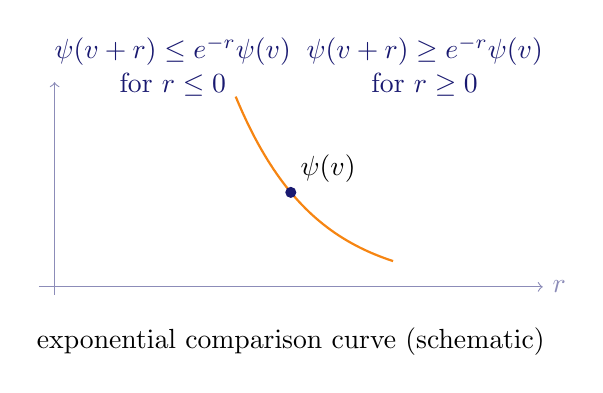
\begin{tikzpicture}[x=1cm,y=1cm]
\draw[->,MidnightBlue!50] (-3.2,0)--(3.2,0) node[right] {$r$};
\draw[->,MidnightBlue!50] (-3,-.1)--(-3,2.6);
\draw[BurntOrange,thick,domain=-.7:1.3,samples=50] plot (\x,{1.2*exp(-\x)});
\fill[MidnightBlue] (0,1.2) circle (2pt);
\node[above right] at (0,1.2) {$\psi(v)$};
\node[align=center,MidnightBlue] at (-1.5,2.8) {$\psi(v+r)\le e^{-r}\psi(v)$\\for $r\le0$};
\node[align=center,MidnightBlue] at (1.7,2.8) {$\psi(v+r)\ge e^{-r}\psi(v)$\\for $r\ge0$};
\node at (0,-.7) {exponential comparison curve (schematic)};
\end{tikzpicture}
